\documentclass[../analysisII_notes.tex]{subfiles}
\begin{document}
\section{Aula 24 - 11 de Junho, 2025}
\subsection{Motivações}
\begin{itemize}
	\item Aplicações das Aplicações Diferenciáveis;
	\item Regra da Cadeia multidimensional.
\end{itemize}
\subsection{Aplicações das Aplicações Diferenciáveis}
Continuaremos com exemplos de aplicações diferenciáveis.
\begin{example}[Coordenadas de uma aplicação diferenciável]
	Seja U um aberto de \(\mathbb{R}^{m}\); então, uma aplicação \(f:U\rightarrow \mathbb{R}^{n}\) é o mesmo que pegarmos n funções reais definidas em U, como \(f_1, f_2,\dotsc , f_{n}:U\rightarrow \mathbb{R}\) como suas coordenadas. Com efeito, fixada a \textit{base canônica} \(\mathcal{B}=\{e_1, e_2, \dotsc , e_{n}\}\) de \(\mathbb{R}^{n}\), para cada x em U, o vetor \(f(x)\) em \(\mathbb{R}^{n}\) se escreve unicamente como
	\[
		f(x)=f_1 (x)e_1 + f_2(x)e_2 + \dotsc + f_{n}(x)e_{n} = (f_1(x), f_2(x), \dotsc , f_{n}(x)),
	\]
	onde \(f_1(x), f_2(x), \dotsc , f_{n}(x)\) são interpretadas como escalares de \(\mathbb{R}\), que são, por definição, as coordenadas do vetor. Logo,
	\[
		f_{i}(x)=\left< f(x), e_{i} \right>.
	\]
	Em particular, se \(T:\mathbb{R}^{m}\rightarrow \mathbb{R}^{n}\) for linear e \(T_1, T_2, \dotsc , T_{n}:\mathbb{R}^{m}\rightarrow \mathbb{R}\) forem suas coordenadas conforme elaborado acima, então para cada h em \(\mathbb{R}^{m}\), vale que
	\[
		T \cdot h = (T_1 \cdot h, T_2 \cdot h, \dotsc , T_n \cdot h)
	\]
	e, além disso, cada \(T_{j}\) é linear. De fato, para todos h, k reais,
	\begin{align*}
		 & T_{i} \cdot h = \left< THh e_{i} \right>                                                                                                                     \\
		 & T_{i}(h+\alpha k) = \left< Th + \alpha Tk, e_{i} \right>= \left< Th, e_{i} \right> + \alpha \left< Tk, e_{i} \right> = T_{i} \cdot h + \alpha T_{i} \cdot k.
	\end{align*}
\end{example}
Com base no exemplo acima,
\begin{prop*}
	Uma função \(f:U\rightarrow \mathbb{R}^{n}\) é diferenciável em um ponto a de U se, e somente se, cada uma de suas coordenadas \(f_1, f_2,\dotsc , f_{n}:U\rightarrow \mathbb{R}\) o for. Além disso, nesse caso,
	\[
		f'(a)\cdot h=(f_1'(a) \cdot h, f_2'(a) \cdot h, \dotsc, f_n'(a) \cdot h), \quad h\in \mathbb{R}^{m}.
	\]
\end{prop*}
\begin{proof*}
	Com efeito, se T é um operador linear de \(\mathbb{R}^{m}\) em \(\mathbb{R}^{n}\), ou seja, \(T\in \mathcal{L}(\mathbb{R}^{m}, \mathbb{R}^{n})\), então a igualdade vetorial
	\begin{align*}
		r(h) & =f(a+h)-f(a)-T \cdot h                                                \\
		     & = (f_1(a+h)-f_1(a)-T_1 \cdot h, \dotsc , f_n(a+h)-f_n(a)-T_n \cdot h)
	\end{align*}


	equivale às n igualdades
	\[
		r_{i}(h)=f_{i}(a+h)-f_{i}(a)-T_{i} \cdot h,\quad i=1, 2, \dotsc , n,
	\]
	de modo que, pela topologia dos espaços euclideanos,
	\[
		\lim_{h\to 0}\frac{r(h)}{|h|}= 0 \Longleftrightarrow \lim_{h\to 0}\frac{r_{i}(h)}{|h|}=0, \quad i=1, 2, \dotsc ,n,
	\]
	portanto provando o resultado. \qedsymbol
\end{proof*}
Conforme vimos na aula passada, se f é derivável em um ponto a de U, então
\[
	f'(a) \cdot h = \lim_{t\to 0}\frac{f(a+th)-f(a)}{t},
\]
tal que
\[
	f_{i}'(a)\cdot h=\lim_{t\to 0}\frac{f_{i}(a+th)-f_{i}(a)}{t}.
\]
Em particular, dados os índices \(i=1,2,\dotsc ,m,\:\&\: j=1,\dotsc ,n\),
\[
	f'(a)\cdot e_{i}=\lim_{t\to 0}\frac{f(a+te_{i})-f(a)}{t}\Rightarrow f_{i}'(a) e_{j}=\lim_{t\to 0}\frac{f_{i}(a+te_{j})-f_{i}(a)}{t},
\]
Sendo assim,
\begin{def*}
	Dada f derivável em um ponto a de U, o limite
	\[
		\frac{\partial^{}f_{i}}{\partial x_{j}^{}}(a)\coloneqq f_{i}'(a) e_{j}=\lim_{t\to 0}\frac{f_{i}(a+te_{j})-f_{i}(a)}{t},\quad i=1,2,\dotsc ,m,\: j=1,\dotsc ,n.
	\]
	é conhecido como \textbf{derivada parcial de \(f_{i}\) com relação à variável} \(x_{j}\). Além disso, o limite
	\[
		f'(a)\cdot h=\frac{\partial^{}f}{\partial h^{}}(a)\coloneqq f_{i}'(a)\cdot h=\lim_{t\to 0}\frac{f_{i}(a+th)-f_{i}(a)}{t}
	\]
	é chamado \textbf{derivada direcional de f no ponto a e na direção do vetor h}. \(\square\)
\end{def*}
Juntando tudo numa ``nova'' notação, podemos escrever
\[
	\frac{\partial^{}f}{\partial h^{}}(a)=\biggl(\frac{\partial^{}f_1}{\partial h^{}}(a), \dotsc , \frac{\partial^{}f_{n}}{\partial h^{}}(a) \biggr) \;\&\; \frac{\partial^{}f}{\partial x_{j}^{}}(a)=\biggl(\frac{\partial^{}f_{1}}{\partial x_{j}^{}}(a), \dotsc , \frac{\partial^{}f_{n}}{\partial x_{j}^{}}(a)\biggr).
\]

\subsection{Regra da Cadeia Multidimensional}
O nosso próximo grande objetivo é provar o teorema da função inversa, que relaciona diferomorfismos -- aplicações diferenciáveis com inversa diferenciável -- com isomorfismos. Um dos resultados que usaremos para isso é que a composta de aplicações diferenciável é uma aplicação diferneciável, que é demonstrado pela regra da cadeia:
\hypertarget{multivariate_chain}{
	\begin{theorem*}[Regra da Cadeia]
		Sejam \(f:U\rightarrow V\) e \(g:V\rightarrow \mathbb{R}^{k}\), tais que
		\begin{itemize}
			\item[i)] U e V são abertos respectivos de \(\mathbb{R}^{m}\) e de \(\mathbb{R}^{n}\);
			\item[ii)] f é diferenciável no ponto a de U; e
			\item[iii)] g é diferenciável em \(b\coloneqq f(a)\) no conjunto V.
		\end{itemize}
		Então, \(g\circ f:U\rightarrow \mathbb{R}^{k}\) é diferenciável em a, e vale a Regra da Cadeia:
		\[
			(g\circ f)'(a) = g'(f(a))\cdot f'(a),
		\]
		ou seja, ``a derivada das compostas é a composta das derivadas''.
	\end{theorem*}
}
\begin{figure}[H]
	\begin{center}
		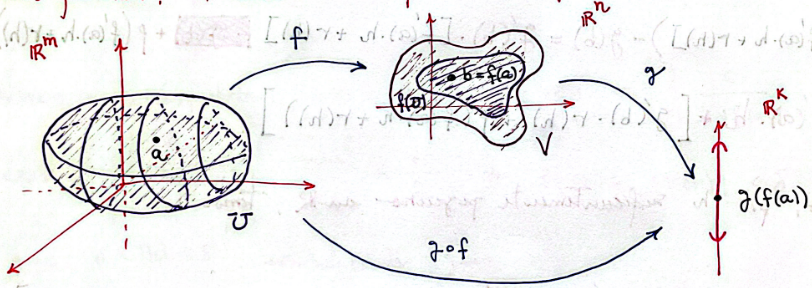
\includegraphics[height=0.6\textheight, width=0.6\textwidth, keepaspectratio]{./Images/chain_rule_24.png}
	\end{center}
	\caption{ilustração visual da regra da cadeia e como ela age num ponto a.}
\end{figure}
\begin{proof*}
	Com efeito, as hipóteses sobre a diferenciabilidade de f e g significam que
	\begin{align*}
		 & r(h) = f(a+h) - f(a) - f'(a) \cdot h     \\
		 & \rho(h) = g(b+s) - g(b) - g'(b) \cdot s,
	\end{align*}
	onde \(b = f(a)\) e elas cumprem, respectivamente,
	\begin{align*}
		 & \lim_{h\to 0}\frac{r(h)}{|h|_{\mathbb{R}^{m}}} = 0  \\
		 & \lim_{s\to 0}\frac{\rho (s)}{|s|_{\mathbb{R}^{n}}}.
	\end{align*}
	Por outro lado, dado h em \(\mathbb{R}^{m}\) suficientemente pequeno, escrevamos
	\[
		(g\circ f)(a+h) - (g\circ f)(a) = g(f(a+h))-g(f(a)),
	\]
	tal que podemos escrever
	\begin{align*}
		g(f(a+h)) - g(f(a)) & = g(f(a)+f'(a)\cdot h+r(h)) - g(f(a)) \\
		                    & = g(b+[f'(a)\cdot h + r(h)]) - g(b).
	\end{align*}
	Como h é pequeno, o valor \(s\coloneqq f'(a)\cdot h + r(h)\) é também pequeno, então podemos dizer que
	\begin{align*}
		g(b+[f'(a)\cdot h+r(h)]) & = g'(b)\cdot [f'(a)\cdot h + r(h)] + \rho(f'(a)\cdot h + r(h))             \\
		                         & = g'(b)\cdot f'(a)\cdot h + [g'(b)\cdot r'(h) + \rho (f'(a)\cdot h+r(h))].
	\end{align*}
	Resumindo, para h suficientemente pequeno em \(\mathbb{R}\), temos:
	\[
		(g\circ f)(a+h) - (g\circ f)(a) = g'(f(a))\cdot f'(a)\cdot h + [g'(b)\cdot r(h) + \rho (f'(a)\cdot h+r(h))],
	\]
	indicando que o resto da aproximação do acréscimo
	\[
		(g\circ f)(a+h) - (g\circ f)(a)
	\]
	pela função linear \(g'(f(a))\cdot f'(a)\) é de fato o que encontramos dentro dos colchetes; assim sendo, para concluirmos o teorema, basta provarmos que
	\[
		\lim_{h\to 0}\frac{g'(b)\cdot r(h) + \rho(f'(a)\cdot h + r(h))}{|h|_{\mathbb{R}^{m}}} = 0.
	\]
	De fato, note que
	\[
		\lim_{h\to 0}\biggl\vert \frac{g'(b)\cdot r(h)}{|h|_{\mathbb{R}^{m}}} \biggr\vert_{\mathbb{R}^{k}}\leq \lim_{h\to 0}\biggl[|g'(b)|_{\mathcal{L}(\mathbb{R}^{n}, \mathbb{R}^{k})}\frac{|r(h)|_{\mathbb{R}^{n}}}{|h|_{\mathbb{R}^{m}}}\biggr] = 0
	\]
	e, como
	\[
		\lim_{s\to 0}\frac{\rho (s)}{|s|} = 0,
	\]
	dado \(\eta > 0\), existe \(\delta \) positivo tal que
	\[
		0 < |s|_{\mathbb{R}^{n}}<\delta \Rightarrow |\rho(s)|_{\mathbb{R}^{k}}\leq \eta |s|_{\mathbb{R}^{n}}.
	\]
	Daí, para esse \(\delta > 0\), corresponde \(\delta'> 0\) de modo que
	\[
		0 < |h|_{\mathbb{R}^{m}}<\delta' \Rightarrow |f'(a)\cdot h + r(h)| < \delta,
	\]
	ou seja,
	\[
		|\rho(f'(a)\cdot h + r(h))|_{\mathbb{R}^{k}}\leq \eta |f'(a)\cdot h + r(h)|_{\mathbb{R}^{n}}.
	\]
	Consequentemente,
	\[
		0 <|h|<\delta' \Rightarrow \biggl\vert \frac{\rho (f'(a)\cdot h + r(h))}{|h|} \biggr\vert\leq |f'(a)\cdot \eta | + \eta \frac{|r(h)|}{|h|}.
	\]
	Nessas condições, dado \(\varepsilon > 0\) e tomando \(\eta \) como
	\[
		0 < \eta < \min\limits_{}\biggl\{\frac{\varepsilon }{2|f'(a)|}, 1\biggr\},
	\]
	existe \(0 < \delta'\) tal que
	\[
		\frac{|r(h)|}{|h|}<\frac{\varepsilon }{2} \;\&\; |f'(a)\cdot h + r(h)|<\delta
	\]
	sempre que \(0 < |h| < \delta'\). Portanto,
	\[
		0 < |h| < \delta ' \Rightarrow \biggl\vert \frac{\rho(f'(a)\cdot h + r(h))}{|h|} \biggr\vert < \frac{\varepsilon }{2} + \frac{\varepsilon }{2} = \varepsilon . \text{ \qedsymbol}
	\]
\end{proof*}
\begin{example}
	Se \(B:\mathbb{R}\times \mathbb{R}\rightarrow \mathbb{R}^{p}\) é bilinear e \(f, g:U\subseteq \mathbb{R}^{m}\rightarrow \mathbb{R}^{n}\) são diferenciáveis no ponto a em U, então \(\varphi :U\rightarrow \mathbb{R}^{p}\) dada por \(\varphi (x) = B(f(x), g(x))\) é diferenciável também no ponto a em U, com
	\[
		\varphi'(a)\cdot h = B(f'(a)\cdot h, g(a)) + B(f(a), g'(a)\cdot h),
	\]
	donde tiramos a conclusão que a regra do produto, ou regra de Leibniz, nada mais é que um caso particular da regra da cadeia multidimensional. Com efeito, para h pequeno em \(\mathbb{R}^{m}\), consideramos o resto
	\[
		r(h) = \varphi (a+h)-\varphi (a)-[B(f'(a)\cdot h, g(a)) + B(f(a), g'(a)\cdot h)]
	\]
	e observemos que
	\begin{align*}
		r(h) & =B(f(a+h), g(a+h)) - B(f(a), g(a)) - B(f'(a)\cdot h, g(a)) - B(f(a), g'(a)\cdot h)   \\
		     & =B(f(a+h), g(a+h)) - B(f(a), g(a+h)) + B(f(a), g(a+h))- B(f(a), g(a))                \\
		     & -- B(f'(a)\cdot h, g(a)) - B(f(a), g'(a)\cdot h)                                     \\
		     & = B(f(a), g(a+h)-g(a)-g'(a)\cdot h) + B(f(a+h)-f(a), g(a+h)) - B(f'(a)\cdot h, g(a)) \\
		     & = B(f(a), g(a+h)-g(a)-g'(a)\cdot h) + B(f(a+h)-f(a)-f'(a)\cdot h, g(a+h)) +          \\
		     & + B(f(a+h) - f(a), g(a+h) - g(a))                                                    \\
		     & = B(f(a), \rho (h)) + B(\sigma (h), g(a)) + B(f(a+h)-f(a), g(a+h)-g(a)).
	\end{align*}
	e das estimativas que uma forma bilinear satisfaz, isto é, para todos x e y em \(\mathbb{R}^{n}\),
	\[
		|B(x, y)|\leq c|x||y|,
	\]
	o fato de termos
	\[
		\lim_{h\to 0}\frac{\rho (h)}{|h|}=0\;\&\; \lim_{h\to 0}\frac{\sigma (h)}{|h|} = 0
	\]
	e de f e g serem contínuas em a, segue a afirmação. \qedsymbol
\end{example}

\end{document}
